\documentclass[conference]{IEEEtran} \IEEEoverridecommandlockouts 
\usepackage[numbers]{natbib} \usepackage{amsmath,amssymb,amsfonts} \usepackage{algorithmic} \usepackage{graphicx} \usepackage{textcomp} \usepackage{xcolor} \usepackage[utf8]{inputenc}\usepackage{float}
 \begin{document} \title{Análisis de Componentes Modelados en LTSpice}
  \author{ \IEEEauthorblockN{Juan Ignacio Caorsi (65532) y Rita Moschini (67026)} \IEEEauthorblockA{Grupo 3} } \maketitle \begin{abstract} 
    En este trabajo se realiza una comparación de los modelos teóricos de componentes mediante simulaciones con LTSpice, analizando el impacto de parámetros no ideales como el coeficiente de emisión en el punto de operación y la caracterización de pequeña señal.
 \end{abstract} \begin{IEEEkeywords} diodo, recta de carga, resistencia estática, resistencia dinámica, factor de idealidad. 
\end{IEEEkeywords}

 \section{Análisis de Diodo} Se planteó un circuito con un diodo en serie con una fuente $V_{CC} = 3,5$ V y una resistencia $R = 10,15$ k$\Omega$. El comportamiento del circuito externo está regido por la recta de carga visible en la Figura \ref{fig:curva_diodo}, derivada de la ley de tensiones de Kirchhoff:
  $ I_D = \frac{V_{CC} - V_D}{R}$. El punto de operación obtenido ($Q$) de la simulación se sitúa en $V_{d}=510,42$ mV e $I_{d}=294,54~\mu$A y se considera que $V_T \approx 25,85$ mV.
   \begin{figure}[htbp] \centering 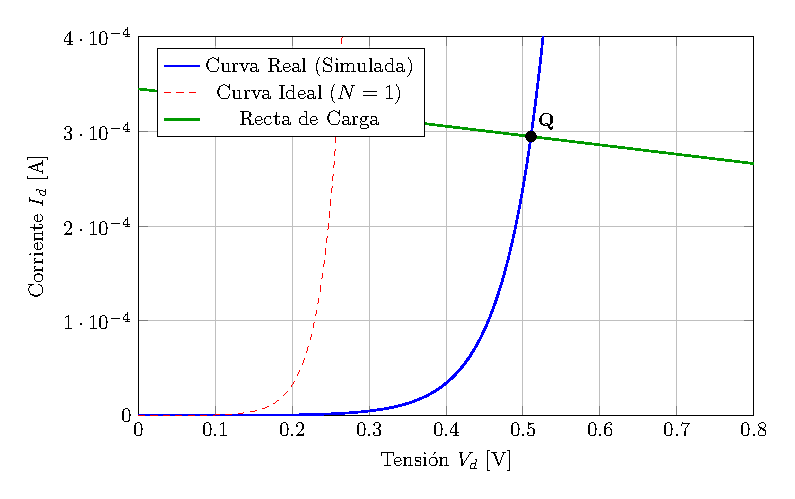
\includegraphics[width=0.5\textwidth]{graficos.pdf} \caption{Curva característica I-V con el punto de operación $Q$ y recta de carga.} \label{fig:curva_diodo} \end{figure} 
   
   A partir del modelo de simulación provisto para el diodo 1N4001, se identificó un coeficiente de emisión $N = 1,984$ y una corriente de saturación $I_s = 14,11$~nA. Según Sedra y Smith \cite{b2}, la presencia de 
   un factor de idealidad cercano a 2 es característica de la "región de baja corriente" ($I_D < 1$ mA), donde predominan los procesos de recombinación
    en la zona de vaciamiento. Dado que el punto $Q$ opera en el orden de los microamperios, este valor de $N$ es fundamental para el ajuste del 
    modelo. \subsection{Parámetros del Modelo (pequeña señal)} Para caracterizar el componente en el punto $Q$, se calcularon las resistencias estática
     ($r_e$) y dinámica ($r_d$). La resistencia estática representa la oposición total al flujo de corriente continua:
      \begin{equation} r_e = \frac{V_D}{I_D} = \frac{510,42 \text{ mV}}{294,54 \text{ }\mu\text{A}} \approx 1,73 \text{ k}\Omega \end{equation} 
      Para el análisis de pequeña señal, se utiliza la resistencia dinámica ($r_d$), que representa la pendiente local de la curva. Utilizando 
      el coeficiente de emisión $N$: \begin{equation} r_d = \frac{N \cdot V_T}{I_D} = \frac{1,984 \cdot 25,85 \text{ mV}}{294,54 \text{ }\mu\text{A}} 
        \approx 174,13 \text{ }\Omega \end{equation} La notable diferencia entre ambos valores ($r_e \approx 10 \cdot r_d$) evidencia la naturaleza 
        no lineal del dispositivo; mientras el diodo presenta una resistencia considerable para establecer el punto de polarización, se comporta 
        como un elemento de baja oposición para variaciones de señal pequeñas en torno a dicho punto. 
    
\section{Análisis del dispositivo JFET (2N3819)}
Estudiaremos un dispositivo JFET con fuentes de tensión $V_{GS} = -1 V$ y $V_{DD}= 20 V$, y una carga de R = 1.8 k $ \Omega$.
    
    \subsection{Punto de Operación Q y Región de Trabajo}
    
    El punto de operación Q en la curva de entrada del JFET de la figura \ref{fig:curvaEntradaJFET} se encuentra determinado por la fuente de tensión $V_{GS}=-1V$ colocada. La simulación mostró que en este punto, $I_D=5.3\,mA$.
    \begin{figure}[H]
        \centering 
        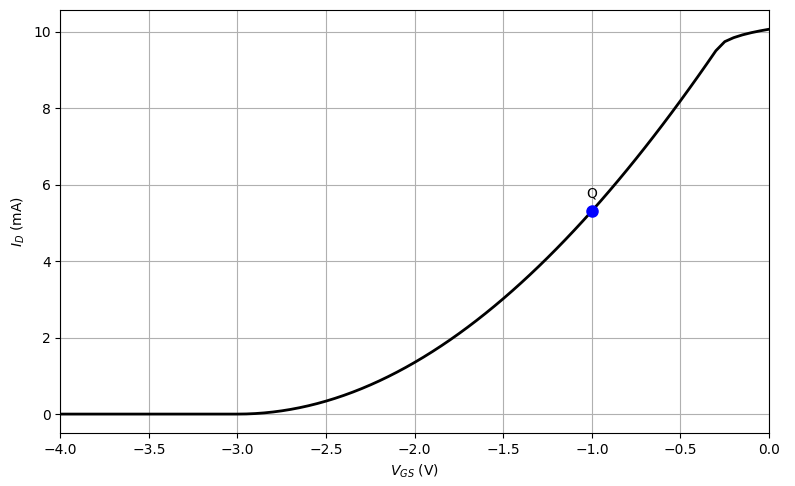
\includegraphics[width=0.4\textwidth]{curvaEntradaJFET.png} 
        \caption{Curva de Entrada del dispositivo JFET.} 
        \label{fig:curvaEntradaJFET}
    \end{figure}
    En la curva de entrada se puede observar 3 "zonas", la primera siendo la zona de corte, que es donde $V_{GS}<V_P$ y $I_D=0\,A$. En este caso, $V_P=-3\,V$ acorde a la simulación de la figura \ref{fig:curvaEntradaJFET} y al modelo del transistor en LTSpice. En la región entre -3 V y -0,25 V la curva presenta un comportamiento aproximadamente cuadrático. Finalmente la zona cercana a $V_{GS}=0\,V$ en la que la corriente $I_D$ se acerca a su valor de saturación $I_{DSS}=10\,mA$.
    \begin{figure}[H]
        \centering 
        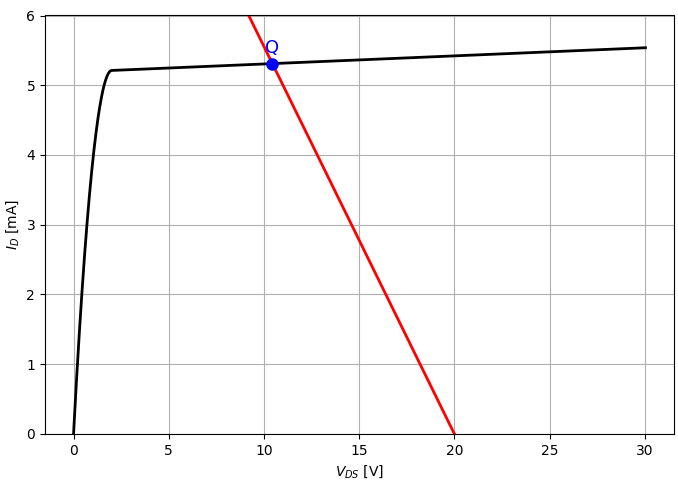
\includegraphics[width=0.4\textwidth]{curvaSalidaJFET.png} 
        \caption{Curva de Salida del dispositivo JFET.} 
        \label{fig:curvaSalidaJFET}
    \end{figure}
    En superposición con la curva de salida del JFET se puede apreciar la recta de carga determinada por $I_D=\frac{V_{DD}-V_{DS}}{R}$. La intersección entre la curva de carga y la curva de salida se encuentra en la región de saturación, de modo que el transistor está polarizado en saturación. Por esto, sabemos que $V_{DS}>V_{DSat}=V_{GS}-V_P=2\,V$.

    
    \subsection{Parámetros del Modelo de Pequeña Señal}
    Se obtuvo un valor para la transconductancia de $g_m=4,44\,mA$. Luego, para calcular la conductancia de salida se calculó la tensión de early $V_A$ a partir del valor de $\lambda=2.25m$ de la simulación, de manera que $V_A=\frac{1}{\lambda}=444,44\,V$. Así, $r_0=\frac{V_A}{I_D}=83.86k\,\Omega$ y $g_d=\frac{I_D}{V_A}=11.92\,\mu\frac{1}{\Omega}$.


\section{Análisis del dispositivo BJT (BC546B )}
    Estudiaremos un dispositivo BJT con fuentes de tensión $V_{BE} = 620\,mV$ y $V_{DD}= 10 V$ y una carga de R = 10 k $ \Omega$.

    El punto de operación Q en la curva de entrada del BJT (figura \ref{fig:curvaEntradaBJT}) se encuentra determinado por la fuente de tensión $V_{GS}=620\,mV$ colocada. La simulación mostró que en este punto, $I_D=523.6\,\mu A$. Dada esta carga, el transistor se encuentra polarizado en modo activo directo. También puedo notar esto porque en mi punto de carga,
    $V_{CE}=V_{DD}-I_C\dot R =10\,V-(523.6\,\mu A)(10\,k\Omega)=4.8\,V $ \\ $V_{BC}=V_{BE}-V_{CE}=620\,mV-4.8V=-4.18\,V<0$.
    Así, dado que $V_{BC}<0$ y $V_{BE}>0$, se obtiene analíticamente que el transistor opera en Modo Activo Directo.
    \begin{figure}[H]
        \centering 
        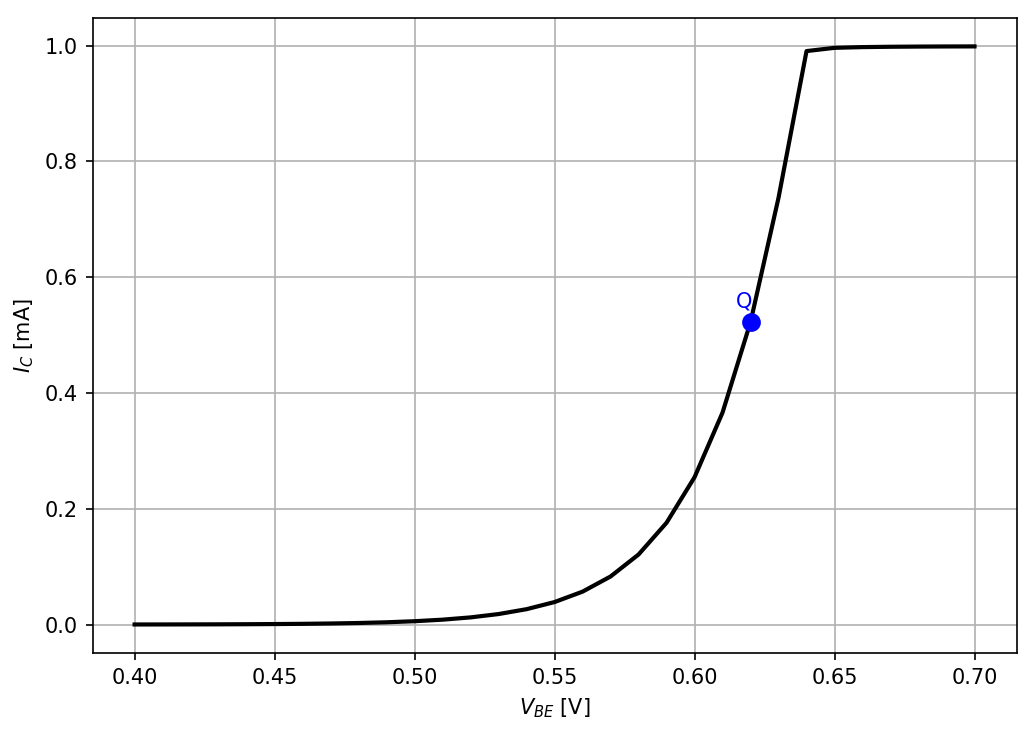
\includegraphics[width=0.4\textwidth]{curvaEntradaBJT.png} 
        \caption{Curva de Entrada del dispositivo BJT.} 
        \label{fig:curvaEntradaBJT}
    \end{figure}
    Por otro lado, en superposición con la curva de salida del BJT se puede apreciar la recta de carga determinada por $I_D=\frac{V_{DD}-V_{CE}}{R}$. La intersección entre la curva de carga y la curva de salida se encuentra en la región en la que el BJT aactúacomo fuente de corriente, es decir en modo activo directo. Otra forma de ver esto es notando que $V_{CE}>V_{CESat}$. Para determinar un valor aproximado de $V_{CESat}$, se observa en la hoja de datos que para $I_C=100\,mA$ e $I_B=5\,mA$, el valor típico de $V_{CESat}$ es 200 mV. A su vez, en el modelo de LTSpice $h_{FE}=\beta=294.3$ (se toma de LTSpice y no de la hoja de datos porque en la hoja de datos hay 3 ganancias según el grupo o tipo del transistor, el cual desconocemos). $I_B=\frac{I_C}{\beta}=1.77\,\mu A$, es decir que la corriente $I_B$ del modelo simulado es todavía menor a $5\,mA$, y el $V_{CESat}$ es todavía menor a 200 mV, por lo que pedir $V_{CE}>V_{CESat}=200 mV$ para que el transistor esté en modo activo directo, asegura que dicha condición se cumpla en el caso modelado.
    \begin{figure}[H]
        \centering 
        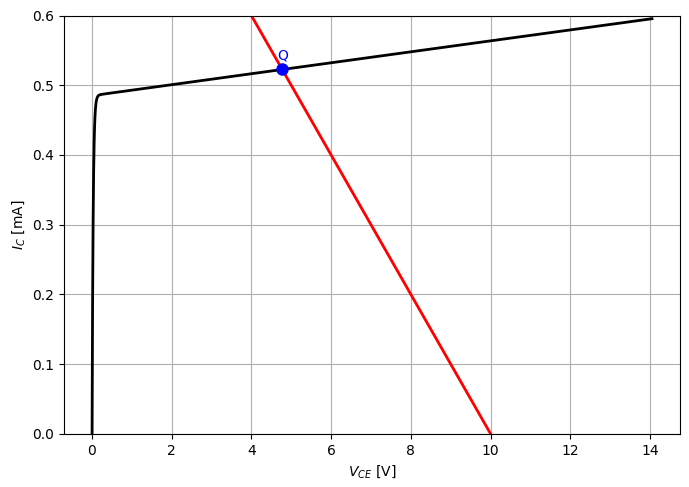
\includegraphics[width=0.4\textwidth]{curvaSalidaBJT.png} 
        \caption{Curva de Salida del dispositivo BJT.} 
        \label{fig:curvaSalidaBJT}
    \end{figure}
    Se puede observar que la curva pasa de saturación a MAD en $V_{CE}=0,15\,V$. El efecto Early es más notorio en el BJT que en el JFET, puesto que la pendiente del tramo horizontal de la curva de salida es mayor para el BJT.
    
    \subsection{Parámetros del Modelo de Pequeña Señal}
    Del modelo de LTSpice obtengo $\beta=294.3$ y $V_A=63.2\,V$. Para $V_T=26\,mV$,  obtengo:
    \begin{table}[H]
        \centering
        \begin{tabular}{|c|c|c|c|} \hline
        $g_m$     & $r_\pi$        & $r_o$           & $r_\mu$ \\   \hline
        20.1 mA/V & 14.6 k$\Omega$ & 120.7 k$\Omega$ & 35.5 M$\Omega$ \\ \hline
    \end{tabular}
    \caption{Parámetros de pequeña señal del BJT.}
    \label{tab:bjtPequenaSenal}
    \end{table}




\section{MOSFET de Enriquecimiento (2N7000)}
Para el análisis del Grupo 3, se configuró un circuito de polarización fija con una resistencia de carga $R_D = 5$ k$\Omega$ y una tensión de alimentación $V_{DD} = 10$ V. La tensión de control aplicada entre puerta y fuente se estableció en $V_{GS} = 1,673$ V.

\subsection{Punto de Operación Q y Región de Trabajo}
A partir de la curva de entrada obtenida mediante la simulación (ver Fig. \ref{fig:mosfet_graficos}), se identificó que el modelo del transistor 2N7000 posee una tensión de umbral $V_{th} = 2,12$ V. Al contrastar este parámetro con la tensión de polarización, se verifica que:  $ V_{GS} (1,673 \text{ V}) < V_{th} (2,12 \text{ V})$.

Dado que la tensión de puerta es insuficiente para inducir la formación del canal de inversión, el dispositivo opera en la \textbf{región de corte}. El punto de operación $Q$ resultante se caracteriza por:
\begin{itemize}
    \item $I_{D,Q} \approx 0$ A: Si bien existen corrientes de subumbral en el orden de los nanoamperios, estas resultan despreciables para el trazado de la recta de carga.
    \item $V_{DS,Q} = V_{DD} - (I_{D,Q} \cdot R_D) \approx 10$ V: Al no haber caída de tensión en $R_D$, el transistor soporta la totalidad de la tensión de fuente.
\end{itemize}

\begin{figure}[htbp]
    \centering
    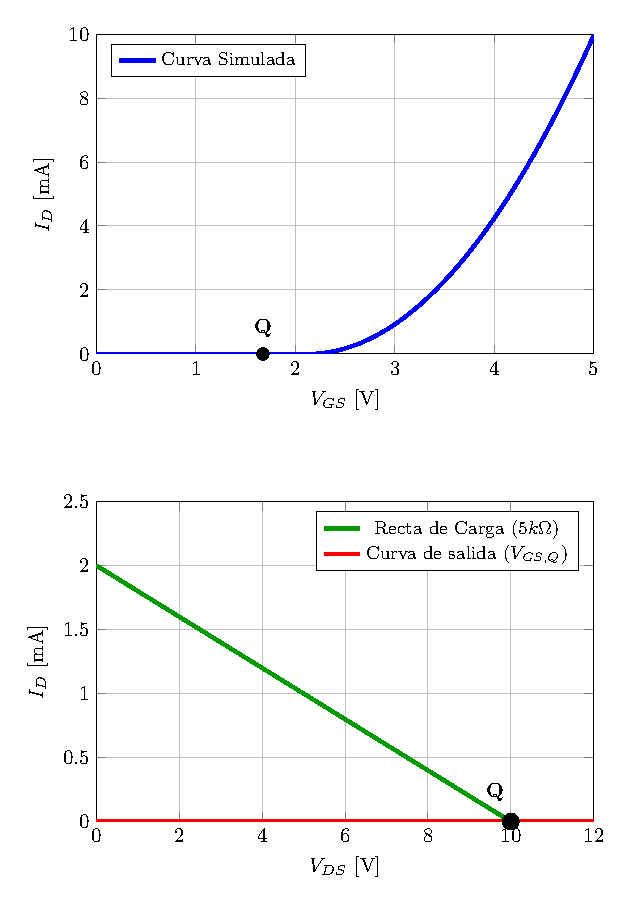
\includegraphics[width=0.45\textwidth]{graficos_mosfet.pdf}
    \caption{Curvas características del MOSFET 2N7000: curva de entrada (arriba) y curva de salida con recta de carga (abajo).}
    \label{fig:mosfet_graficos}
\end{figure}

\subsection{Parámetros de Pequeña Señal}
En la región de corte, la pendiente de la curva de salida es nula, lo que implica que el dispositivo no presenta capacidad de amplificación ni respuesta ante variaciones de señal en este punto:
\begin{itemize}
    \item \textbf{Transconductancia ($g_m$):} $0$ mA/V. 
    \item \textbf{Resistencia de salida ($r_o$):} Teóricamente infinita, el componente se comporta como un circuito abierto entre drenaje y fuente.
\end{itemize}






\section{MOSFET de Vaciamiento (LND150h)}
Se analizó el MOSFET de vaciamiento LND150h con una resistencia de carga $R_D = 8,5$ k$\Omega$ y $V_{DD} = 10$ V. La tensión de polarización se fijó en $V_{GS} = 0,3$ V.




\subsection{Punto de Operación Q y Región de Trabajo}
A partir del modelo SPICE proporcionado, se identifica una tensión de umbral $V_{to} = -1,4$ V y un parámetro $K_p = 3$ mA/V$^2$. Dado que $V_{GS} > V_{to}$ ($0,3 \text{ V} > -1,4 \text{ V}$), el dispositivo se encuentra en conducción.

Utilizando la ecuación cuadrática ideal de saturación:
\begin{equation}
    I_D = \frac{K_p}{2} (V_{GS} - V_{to})^2 = \frac{3 \text{ mA/V}^2}{2} (0,3\text{V} - (-1,4\text{V}))^2 
\end{equation}

Obteniendo finalmente $\approx 4,33 \text{ mA}$. Sin embargo, al considerar la recta de carga:
\begin{equation}
    V_{DS} = V_{DD} - I_D \cdot R_D = 10\text{V} - (I_D \cdot 8,5\text{k}\Omega)
\end{equation}

 Si la corriente fuera de $4,33$ mA, $V_{DS}$ sería negativo, lo cual es físicamente imposible. Esta discrepancia demuestra que el elevado valor de la resistencia externa $R_D$ absorbe la mayor parte del tensión de la fuente, limitando la corriente máxima y forzando al dispositivo a operar en la \textbf{región óhmica o de triodo}. Por su parte, las resistencias parásitas e imperfecciones internas del modelo \texttt{VDMOS} en SPICE terminan de realizar el ajuste fino sobre el valor exacto de dicha corriente. Realizando la simulación (ver Fig. \ref{fig:mosfet_dep_graficos}), se obtuvo
\begin{itemize}
    \item $I_{D,Q} \approx 1,12$ mA
    \item $V_{DS,Q} \approx 0,48$ V
\end{itemize}




\subsection{Parámetros de Pequeña Señal}
En la región de triodo, los parámetros se definen por la pendiente de la curva en una zona de baja resistencia:
\begin{itemize}
    \item \textbf{Transconductancia ($g_m$):} $K_p \cdot V_{DS} \approx 3 \text{ mA/V}^2 \cdot 0,48 \text{ V} = 1,44$ mA/V.
    \item \textbf{Resistencia de salida ($r_{ds}$):} En triodo es baja, aproximadamente $1 / [K_p(V_{GS} - V_{to})] \approx 196 \Omega$.
\end{itemize}

\begin{figure}[htbp]
    \centering
    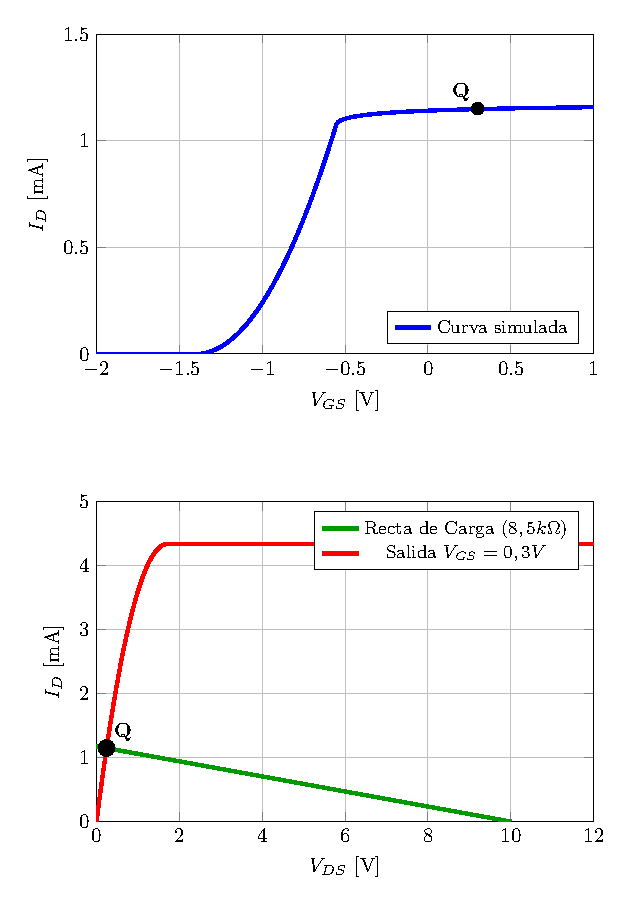
\includegraphics[width=0.45\textwidth]{graficos_lnd150.pdf}
    \caption{Curvas para el LND150h: entrada (arriba) y Salida (abajo). El punto Q se ubica en la región de triodo debido al alto valor de $R_D$.}
    \label{fig:mosfet_dep_graficos}
\end{figure}




\subsection{Análisis Comparativo}
Este resultado resulta llamativo al compararlo con el modelo de vaciamiento. Mientras que el LND150 conduce con $V_{GS}=0$V, el 2N7000 requiere una excitación significativamente mayor para salir del estado de reposo. En la hoja de datos, el rango de $V_{th}$ puede ser tan bajo como $0,8$ V; si se utilizara un componente físico con ese valor mínimo, el transistor estaría en conducción, lo que demuestra la alta sensibilidad del diseño al componente específico seleccionado.
\par Por otro lado, se puede observar que la pendiente de la curva de salida del MOSFET de vaciamiento LND150H es prácticamente nula, es decir que la aproximación Early sobre este dispositivo es despreciable.

        \section{Conclusiones} La inclusión del c
        oeficiente de emisión en el cálculo de la resistencia dinámica permite un ajuste preciso con los resultados de simulación. Se verificó 
        que el modelo de diodo ideal subestima significativamente la $r_d$ en regímenes de baja corriente, lo que afectaría la ganancia en un 
        diseño de amplificación real. \begin{thebibliography}{00} \bibitem{b2} A. S. Sedra y K. C. Smith, \textit{Microelectronic Circuits}, 7ma ed. Oxford University 
            Press, 2015, Cap. 4. \end{thebibliography} \end{document}